\chapter{Przetwarzanie danych zebranych z odbiorników}

W ramach pracy powstało oprogramowanie uruchamiane na komputerze, którego zadaniem jest
przekształcenie surowych danych ultradźwiękowych 
z odbiornika na położenie nadajnika w przestrzeni oraz jego orientację.
Oprogramowanie podzielone zostało na trzy części: bibliotekę \textit{mp3d} zajmującą się
sterowaniem odbiornika, odbieraniem sygnałów ultradźwiękowych i ich analizą, program \textit{scan.py}
wizualizujący dane w postaci obrazu trójwymiarowego oraz program \textit{save-pattern.py},
który służy do wstępnej kalibracji urządzenia.


Najistotniejszą częścią oprogramowania stanowi biblioteka \textit{mp3d}, została ona podzielona na pięć modułów:
\begin{enumerate}
 \item \textit{com.py} - moduł odpowiedzialny za komunikację z odbiornikiem
 \item \textit{find\_pattern.py} - moduł odpowiedzialny za wyznaczanie odległości poprzez wyszukanie wzorca w odebranym sygnale
 \item \textit{xyz.py} - moduł odpowiedzialny za wyznaczenie pozycji i orientacji nadajnika oraz za 
 weryfikację, czy zebrane dane odpowiadają modelowanej rzeczywistości
 \item \textit{info.py} - moduł wyświetlający informację o sile odbieranego sygnału
 \item \textit{ply.py} - moduł odpowiedzialny za eksportowanie danych do formaty \textit{.ply} 
    (Polygon File Format) obsługiwanego przez większość programów do obróbki grafiki 3D.
\end{enumerate}


\section{Komunikacja z odbiornikiem, moduł \textit{com.py}}

Za komunikację z odbiornikiem odpowiedzialny jest moduł \textit{com.py},
pracuje on w oddzielnym wątku, w którym cyklicznie wysyłane są żądania by dany głośnik nadał sygnał,
następnie odbierane są sygnały z trzech mikrofonów.
Ta czynność powtarzana jest dla każdego z czterech głośników nadajnika.
Zebrane dwanaście sygnałów po wstępnej filtracji przekazywane są dalej do \textit{find\_pattern.py}. Cały cykl powtarzany jest
co \SI{350}{ms}. Na rysunku \ref{fig:com_output_2m} przedstawiono odebrany sygnał z jednego mikrofonu.


\begin{figure}[h!]
    \centering
    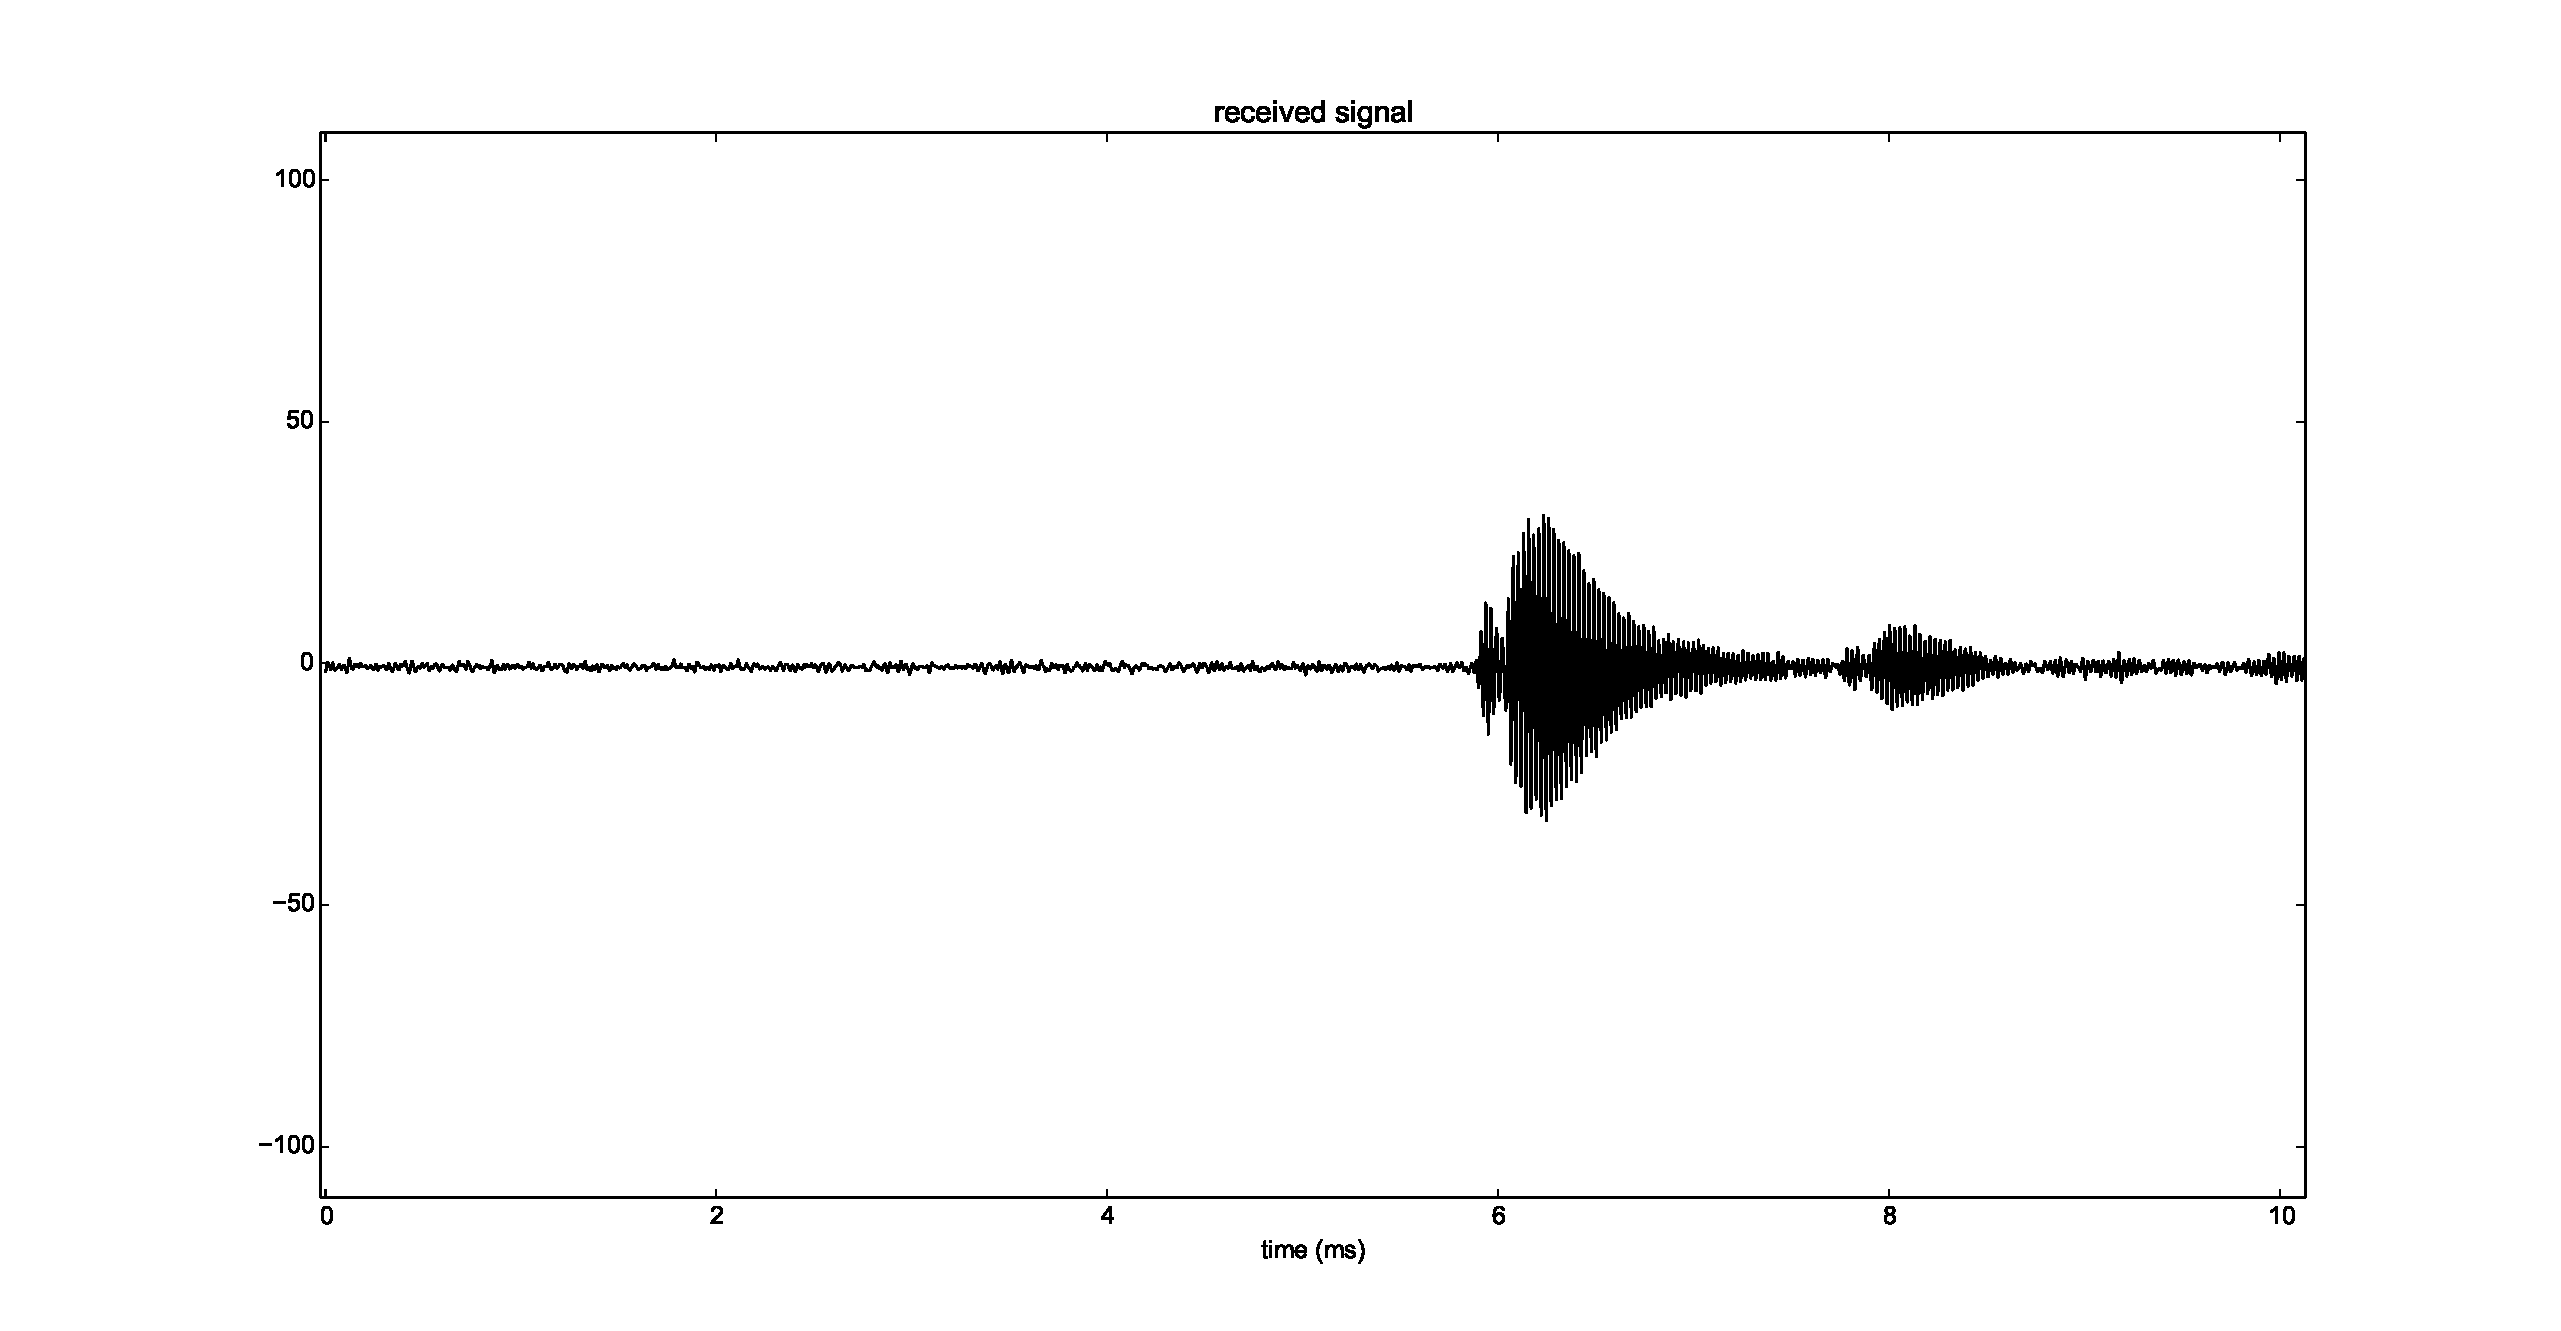
\includegraphics[width=1.15\textwidth, trim= 47mm 0mm 0mm 0mm,clip]{com_output_2m_1}
    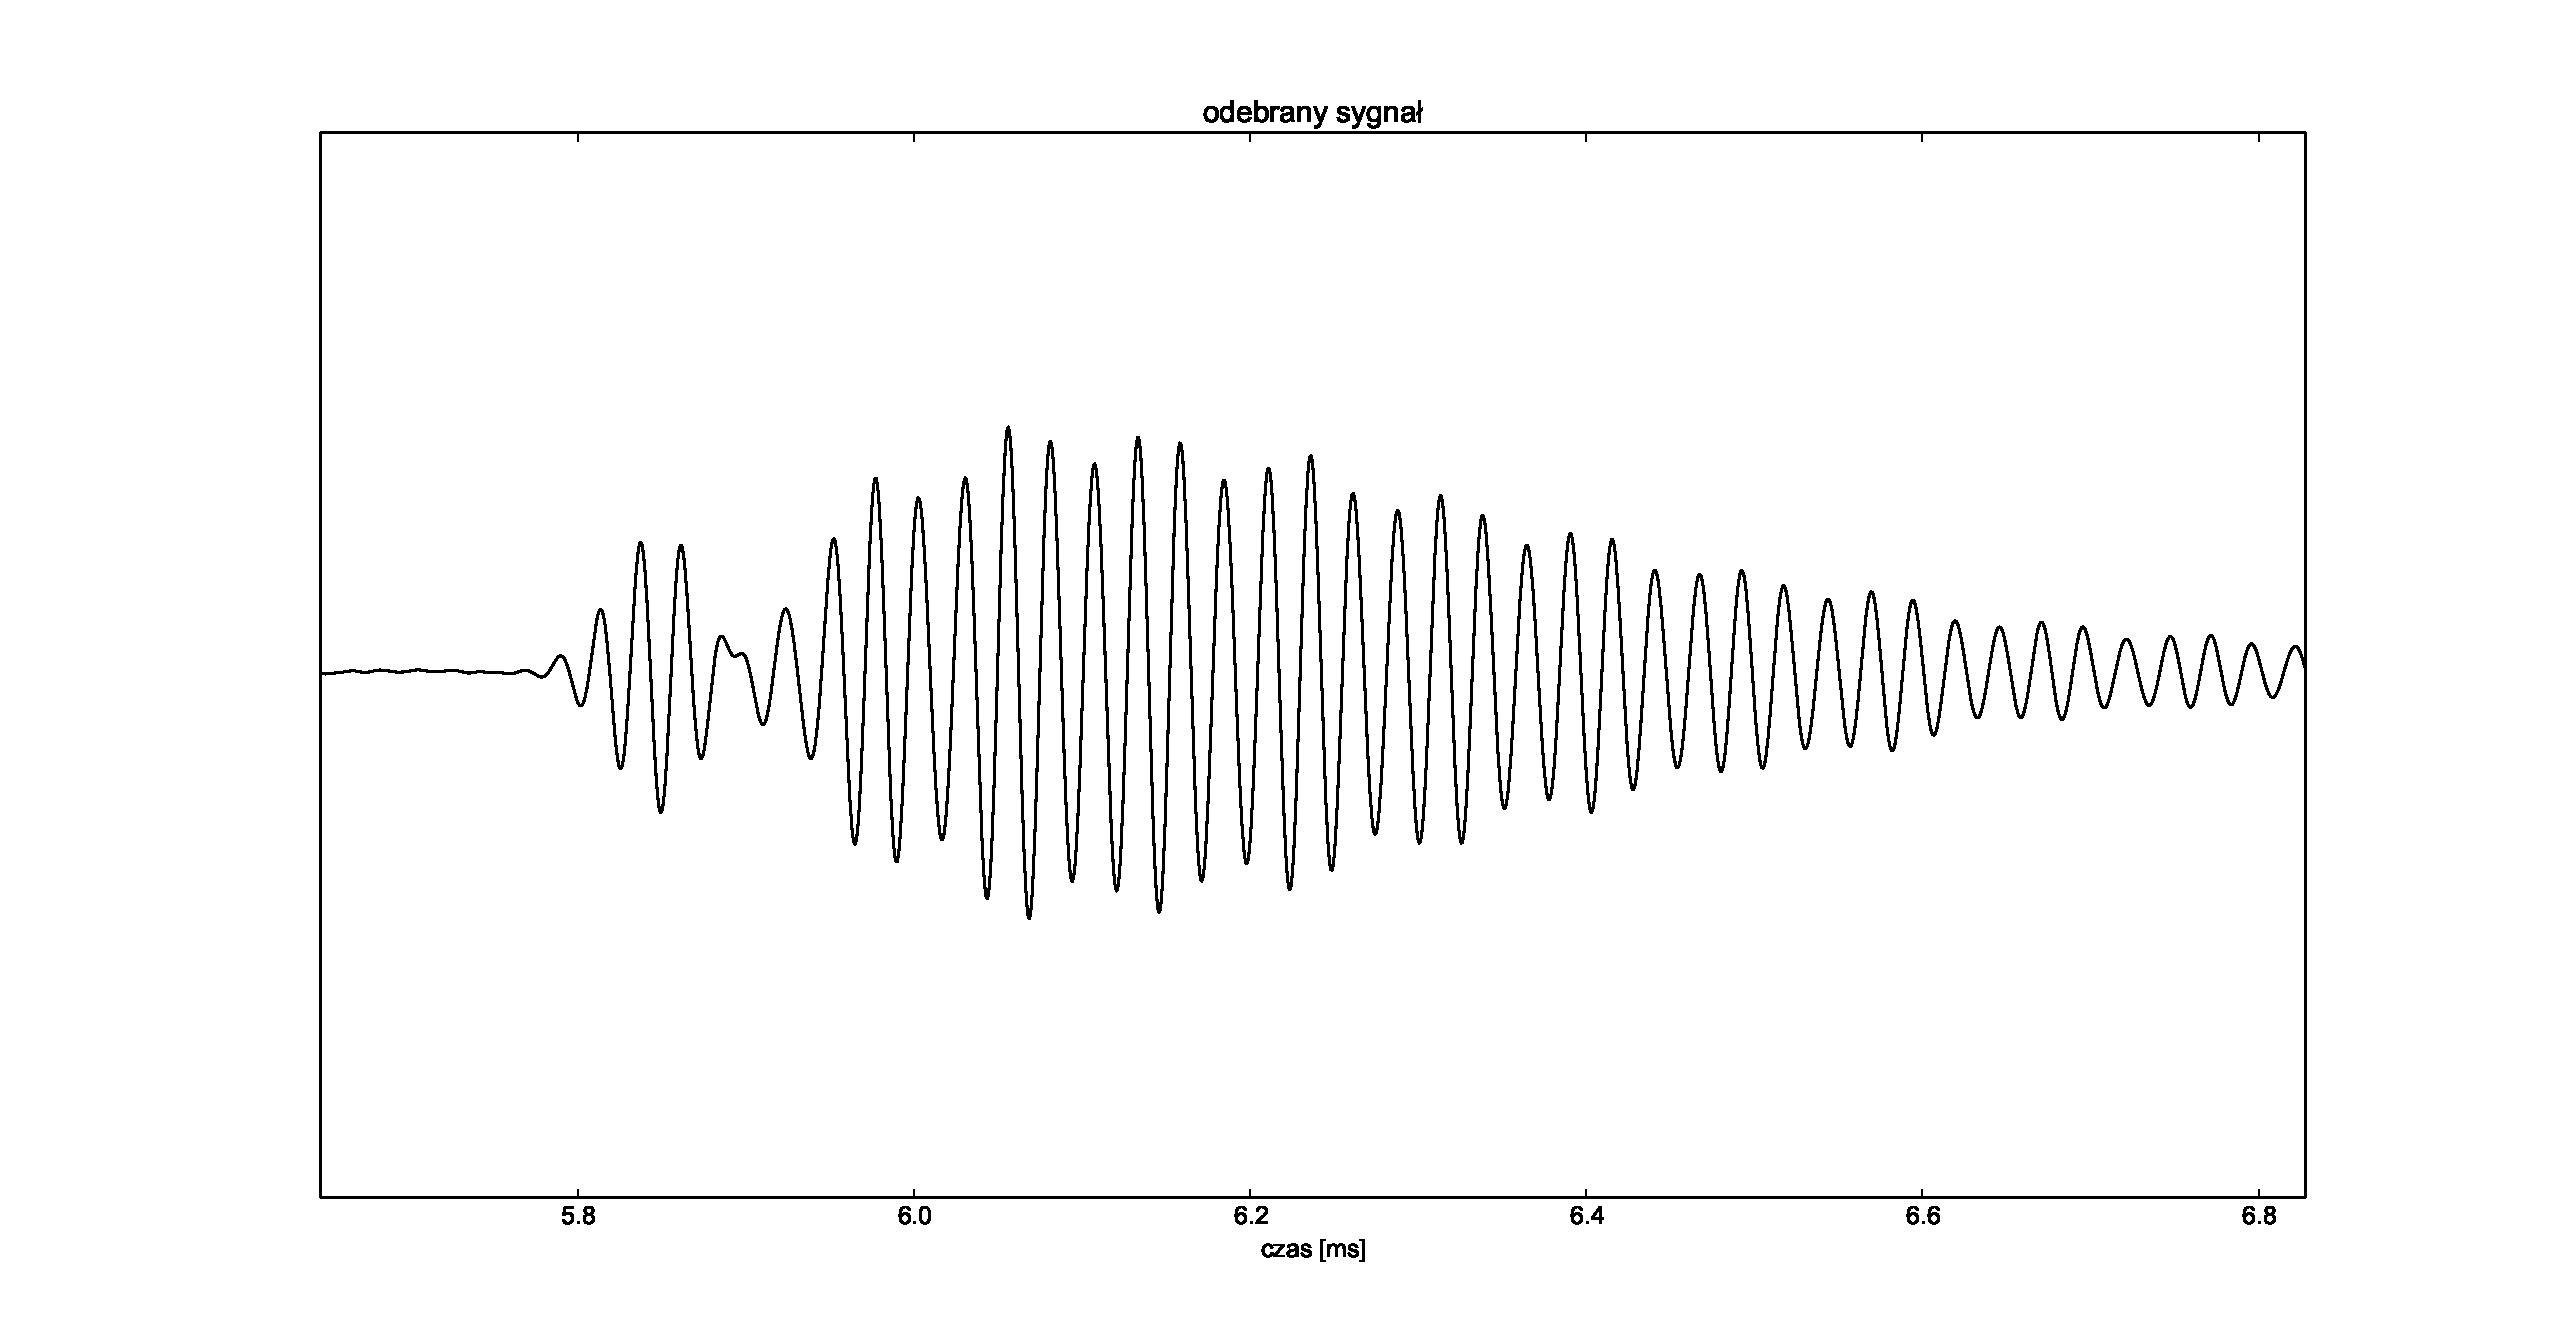
\includegraphics[width=1.15\textwidth, trim= 47mm 0mm 0mm 0mm,clip]{com_output_2m_2}
    \caption{Sygnał odebrany przez moduł \textit{com.py}. 
    Odległość między nadajnikiem a odbiornikiem wynosi 2 metry.
    Na górnym wykresie po prawej stronie widoczne są również sygnały odbite od ścian.
    }
    \label{fig:com_output_2m}
\end{figure}


\section{Wyznaczanie odległości, moduł \textit{find\_pattern.py}}

Moduł \textit{find\_pattern.py} odpowiada za obliczenie odległości pomiędzy czterema głośnikami i trzema mikrofonami.
Odległość wyznaczana jest poprzez wyszukanie położenia \textit{wzorca} odpowiadającego czołu nadanego sygnału 
w każdym z 12 odebranych sygnałów (rysunek \ref{fig:com_output_2m}).
\textit{Wzorzec} początkowo wprowadzany jest podczas kalibracji, następnie jest ciągle aktualizowany 
(podmieniany z sygnałem pasującym do \textit{wzorca}).

Do wyszukania \textit{wzorca} wewnątrz sygnału wykorzystana jest metoda najmniejszego błędu średniokwadratowego:

niech $w(t)$  dla $t = 0..n-1$ będzie szukanym \textit{wzorcem}, a $f(x)$ odebranym sygnałem,
wtedy możemy znaleźć takie $a$, że błąd średniokwadratowy $E(x)$ pomiędzy $w(t)$ i $a f(t+x)$ jest minimalny,
możemy to zapisać w postaci:
\[
  E(x) = \min_{a \in R} \{ \sum_{t=0}^{n-1}  (w(t) - a f(t+x))^2 \}
\]
po podniesieniu wyrażenia w nawiasie do kwadratu otrzymujemy:
\[
  E(x) = \min_{a \in R} \{ \sum_{t=0}^{n-1}  (w^2(t) -2a w(t) f(t+x) + a^2 f^2(t+x)) \}
\]
\[
  E(x) = \min_{a \in R} \{ \sum_{t=0}^{n-1}  w^2(t) -2a \sum_{t=0}^{n-1}  w(t) f(t+x) + a^2 \sum_{t=0}^{n-1} f^2(t+x) \}
\]
aby wyliczyć $E(x)$ należy zminimalizować wyrażenie:
\[
  y(a) = \sum_{t=0}^{n-1}  w^2(t) -2a \sum_{t=0}^{n-1}  w(t) f(t+x) + a^2 \sum_{t=0}^{n-1} f^2(t+x)
\]
 korzystając z faktu, że $y(a)$ jest funkcją kwadratową, możemy wyliczyć $a$ minimalizujące $y(a)$:
\[
 a = \frac{ \sum\limits_{t=0}^{n-1}  w(t) f(t+x) }{ \sum\limits_{t=0}^{n-1} f^2(t+x) }
\]
ostatecznie dostajemy wzór na $E(x)$:
\[
  E(x) = \sum_{t=0}^{n-1}  w^2(t)  - \frac {(\sum\limits_{t=0}^{n-1}  w(t) f(t+x) )^2 } { \sum\limits_{t=0}^{n-1} f^2(t+x)}
\]

Zauważmy, że dzięki skalowaniu sygnału $f(x)$ zamiast \textit{wzorcowa} $w(x)$
otrzymany błąd $E(x)$ nie zależy od siły odebranego sygnału co ułatwia porównanie błędów w dwóch różnych miejscach,
zależy on jednak od siły sygnału wzorcowego, aby się od niego uniezależnić możemy wyznaczyć
błąd względny $e(x)$:
\[
  e(x) = \frac{E(x)}{\sum\limits_{t=0}^{n-1}  w^2(t)}
\]
po podstawieniu $E(x)$ dostajemy:
\[
  e(x) = 1 - \frac {(\sum\limits_{t=0}^{n-1}  w(t) f(t+x) )^2 } { \sum\limits_{t=0}^{n-1} f^2(t+x) \sum\limits_{t=0}^{n-1}  w^2(t)}
\]
 
 Funkcję $e(x)$  można interpretować jako:
 im mniejszy błąd $e(x)$ tym większe prawdopodobieństwo, że szukany wzorzec $w$ znajduje się na pozycji $x$ w 
 odebranym sygnale $f$. 

 Wynikiem obliczeń modułu \textit{find\_pattern.py} jest cała funkcja $e(x)$, na podstawie której moduł \textit{xyz.py}
 wyznaczy pozycję głowicy w przestrzeni jak i jego orientację uwzględniając przy tym 
 kształt głowicy (nadmiarowość danych) jak i prawdopodobieństwo że znaleziony wzorzec jest na danej pozycji.
 Na rysunku \ref{fig:blad_korel} przedstawiono wynik przetwarzania sygnału poprzez moduł \textit{find\_pattern.py}.

\begin{figure}[h!]
    \centering
    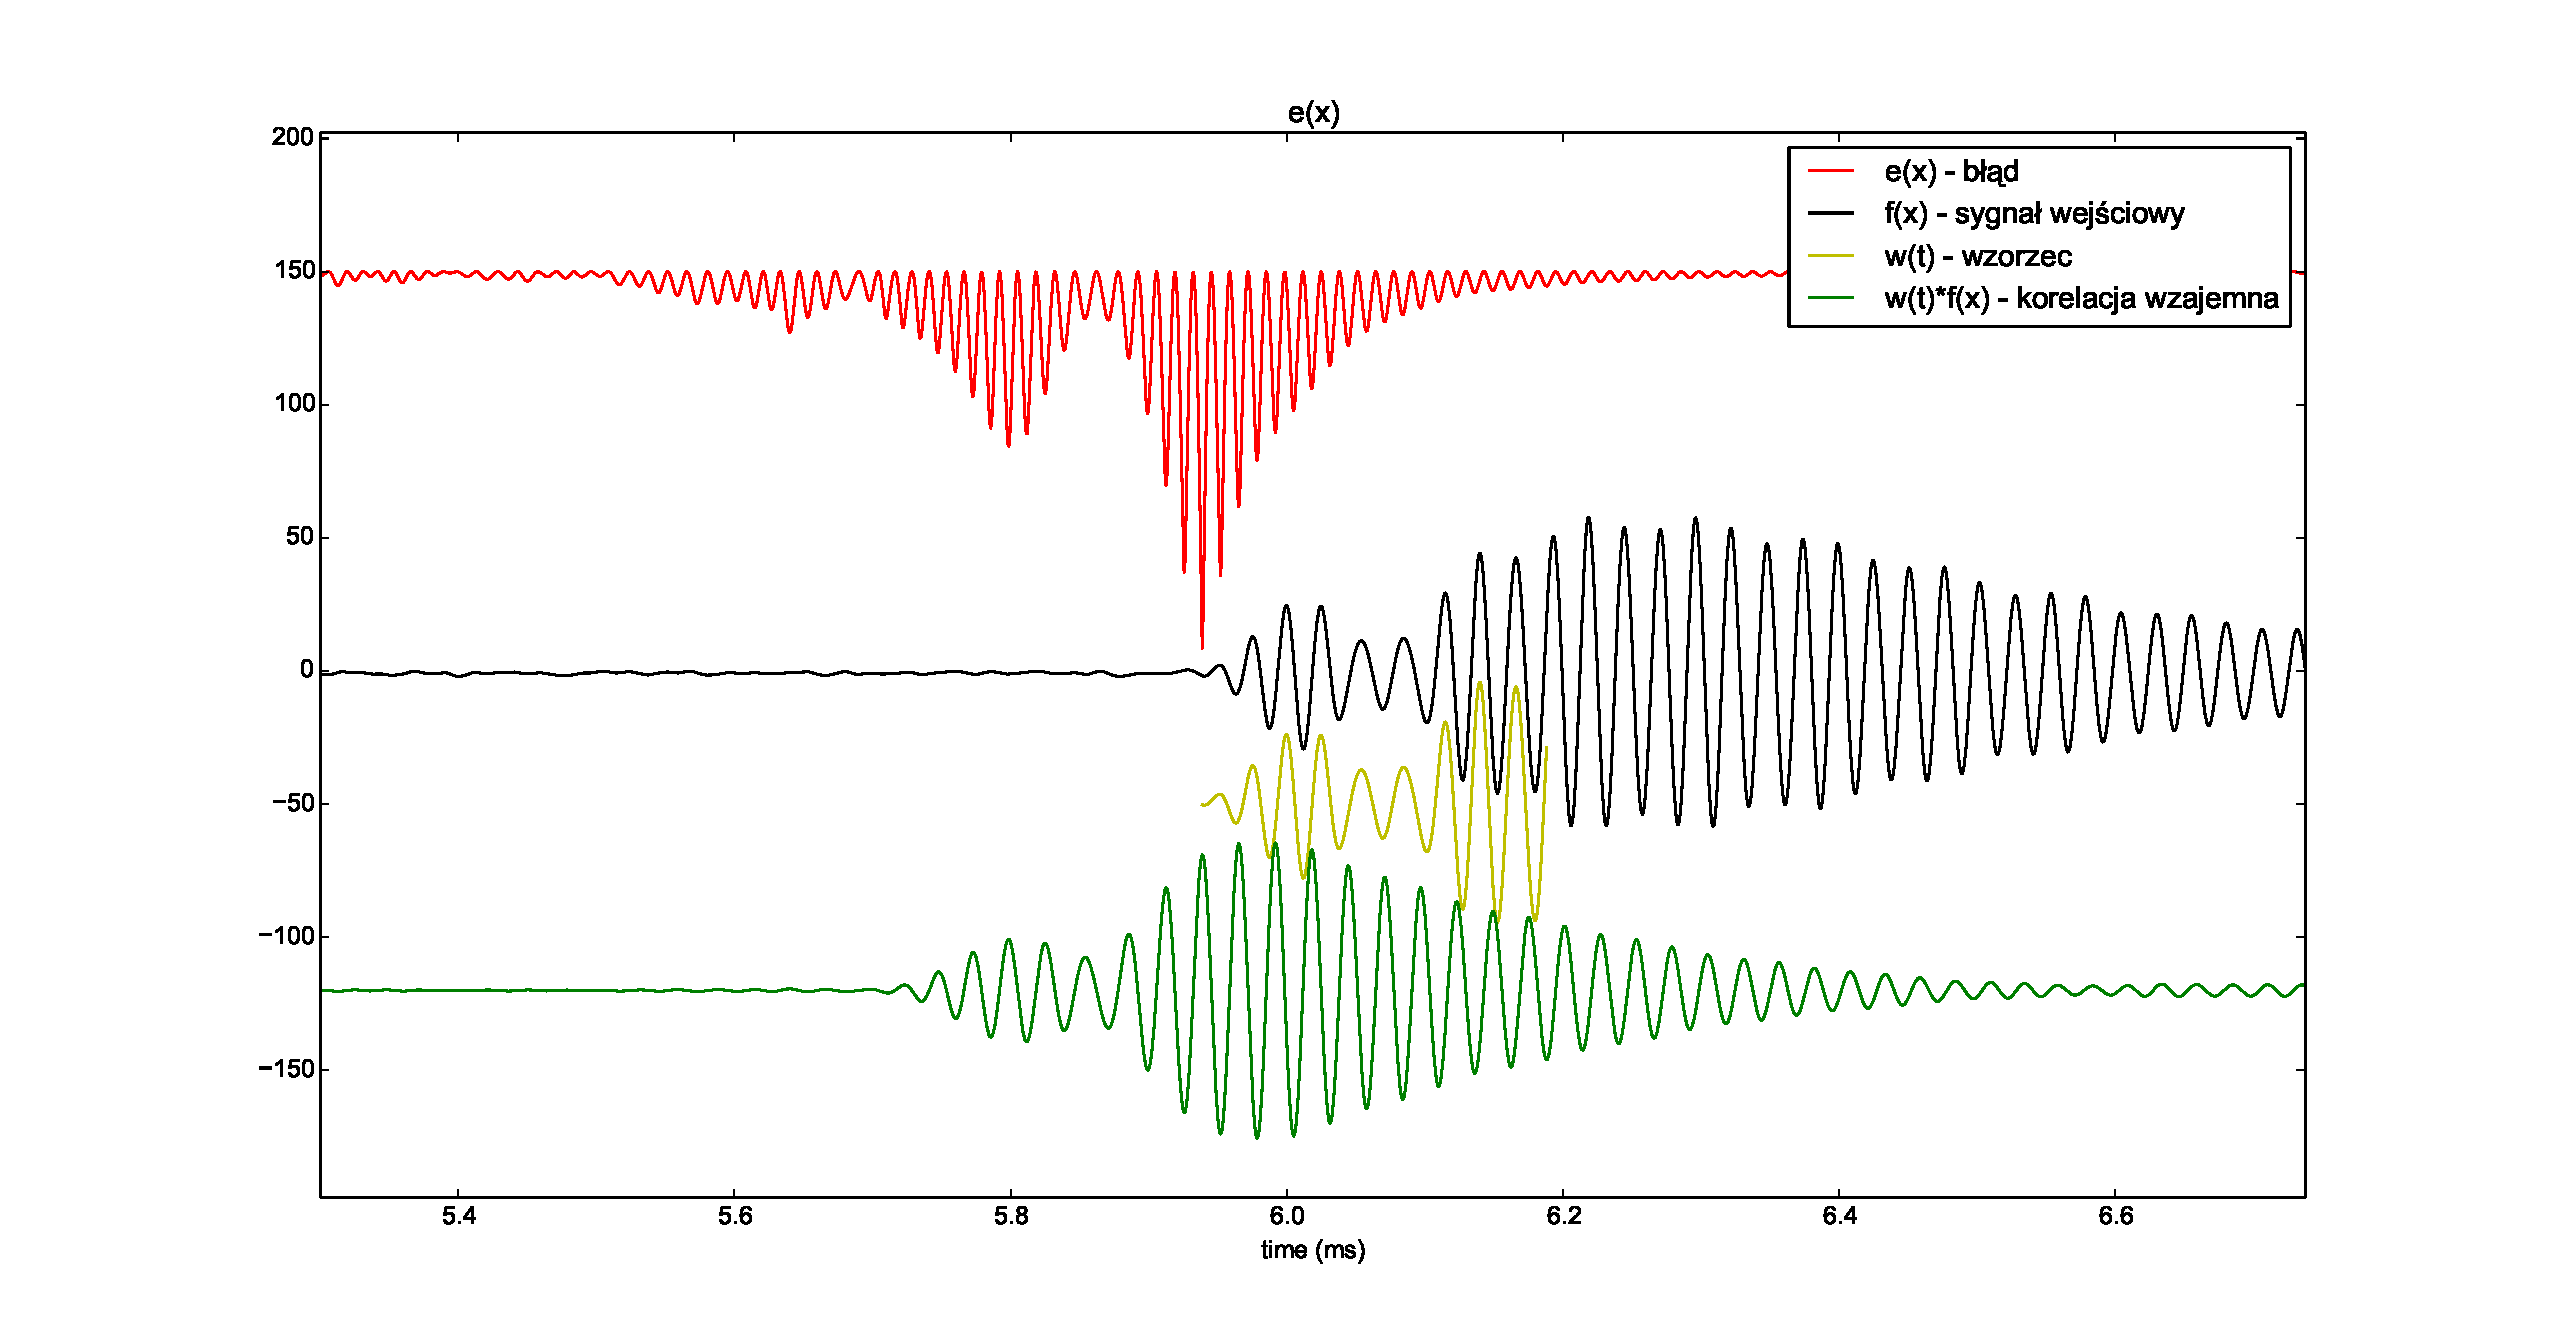
\includegraphics[width=1.15\textwidth, trim= 47mm 0mm 0mm 0mm,clip]{blad_korel}
    \caption{Sygnał przetworzony przez moduł \textit{find\_pattern.py}.}
    \label{fig:blad_korel}
\end{figure}
 
 
 Analiza złożoności obliczeniowej: wyliczenie $ \sum\limits_{t=0}^{n-1}  w^2(t) $ 
jak i $\sum\limits_{t=0}^{n-1} f^2(t+x)$ wymaga jedynie liniowej liczby operacji, a 
 $\sum\limits_{t=0}^{n-1}  w(t) f(t+x) $ jest korelacją wzajemną funkcji $w(t)$ i $f(x)$, którą
 można wyliczyć w czasie $m \log(m)$ korzystając z szybkiej transformacji Fouriera \cite{bib:FFT_correlation},
 gdzie $m = \max \{|w|, |f| \}$, czyli wyliczenie całej funkcji $e(x)$ wymaga jedynie $m \log(m)$ operacji.

 
 Kolejnym zadaniem modułu \textit{find\_pattern.py} jest uaktualnianie \textit{wzorca}.
 Wraz ze zmianą kąta nachylenia nadajnika względem odbiornika zmienia się kształt odbieranego sygnału,
 dlatego jeśli badany sygnał zawiera szukany \textit{wzorzec} oraz spełnione są następujące warunki:
 \begin{itemize}
  \item moc sygnału pasującego do \textit{wzorca} jest wystarczająco duża
  \item błąd względny pomiędzy sygnałem a \textit{wzorcem} jest mały
  \item moduł \textit{xyz.py} "uzna", że otrzymane pozycje pasują do modelowanej rzeczywistości
 \end{itemize}
to moduł uaktualni \textit{wzorzec}.
  
 
\section{Wyznaczanie pozycji oraz orientacji przestrzennej, moduł \textit{xyz.py}}

Ostatnim etapem obliczeń jest wyznaczenie współrzędnych kartezjańskich czterech głośników znajdujących się na nadajniku,
na podstawie których obliczana jest pozycja jaki i orientacja całego nadajnika.
Tym etapem zajmuje się moduł \textit{xyz.py}. Moduł zawiera również prosty model rzeczywistości,
którego celem jest wyłapanie niepoprawnych danych o położeniu.
Niepoprawne dane powstają gdy część głośników traci widoczność z mikrofonami np. gdy zostaną przysłonięte.
W ramach modelowanej rzeczywistości wyliczane są:
\begin{itemize}
  \item prędkość z jaką porusza się każdy z głośników
  \item kształt nadajnika - położenie głośników względem siebie w przestrzeni
\end{itemize}
Jeśli któreś z wyliczeń odbiega od z góry ustalonej normy to dany pomiar uznawany jest za nieprawidłowy.


Współrzędne głośników wyznaczane są na podstawie dwunastu funkcji $e_{ij}(x)$ dla $i=1, ..., 4$ i $j=1, ..., 3$,
które zawierające informację o odległości pomiędzy głośnikiem $i$ oraz mikrofonem $j$.
Dla każdej funkcji $e_{ij}(x)$ wyszukiwane są pozycje minimów lokalnych tych funkcji, 
z których następnie wybierane jest $t$ pozycji $x^{ij}_1, ..., x^{ij}_t$
o najmniejszych wartościach, gdzie $t$ jest stałą wewnętrzną modułu \textit{xyz.py}.
Pozycje te są odległościami, dla których błąd średniokwadratowy
$e_{ij}(x^{ij}_k)$ dla $k=1, ..., t$ pomiędzy szukanym sygnałem (\textit{wzorcem}), a odebranym sygnałem na pozycji $x^{ij}_k$
jest lokalnym minimum jak i jest mały w sensie globalnym,
pozycje $x^{ij}_k$ można również  interpretować jako najbardziej prawdopodobne odległości pomiędzy głośnikiem, a mikrofonem.

Do wyliczenia położenia głośników w przestrzeni wykorzystywane są wszystkie możliwe kombinacje wyznaczonych odległości,
zauważmy że jest ich $12^t$. Każda z możliwych kombinacji 
sprawdzana jest czy jest akceptowalna dla modelowanej rzeczywistości, z tych które są akceptowalne wybierana jest 
kombinacja o najmniejszym sumarycznym błędzie średniokwadratowym, czyli najbardziej prawdopodobna.

Ostatecznym wynikiem  moduły \textit{xyz.py} są wartości $x^{ij}$, czyli najbardziej prawdopodobne odległości
pomiędzy  $i$-tym głośnikiem (gdzie $i=1,...,4$), a $j$-tym mikrofonem, na podstawie których 
wyznaczana jest pozycja oraz orientacja nadajnika.

Wartości $x^{ij}$ przekazywane są również z powrotem do moduły \textit{find\_pattern.py} w celu aktualizacji \textit{wzorców}.


\section{Kalibracja}

Przed każdym uruchomieniem urządzenia wymagana jest kalibracja,
która sprowadza się do ustawienia nadajnika w odległości 2 metrów od odbiornika,
uruchomienia programu \textit{save-pattern.py} oraz zaznaczenia w nim 12 obszarów w odebranym sygnale czoło odebranego sygału.
Obszary te wykorzystane zostaną jako \textit{wzorce} podczas mierzenia odległości.
Program wyliczy również aktualną prędkość dźwięku uwzględniając odległość nadajnika od odbiornika.

Rysunek \ref{fig:kalibracja_12x} przedstawia widok 12 sygnałów wraz z zaznaczonymi wzorcami.


 \begin{figure}[h!]
    \centering
    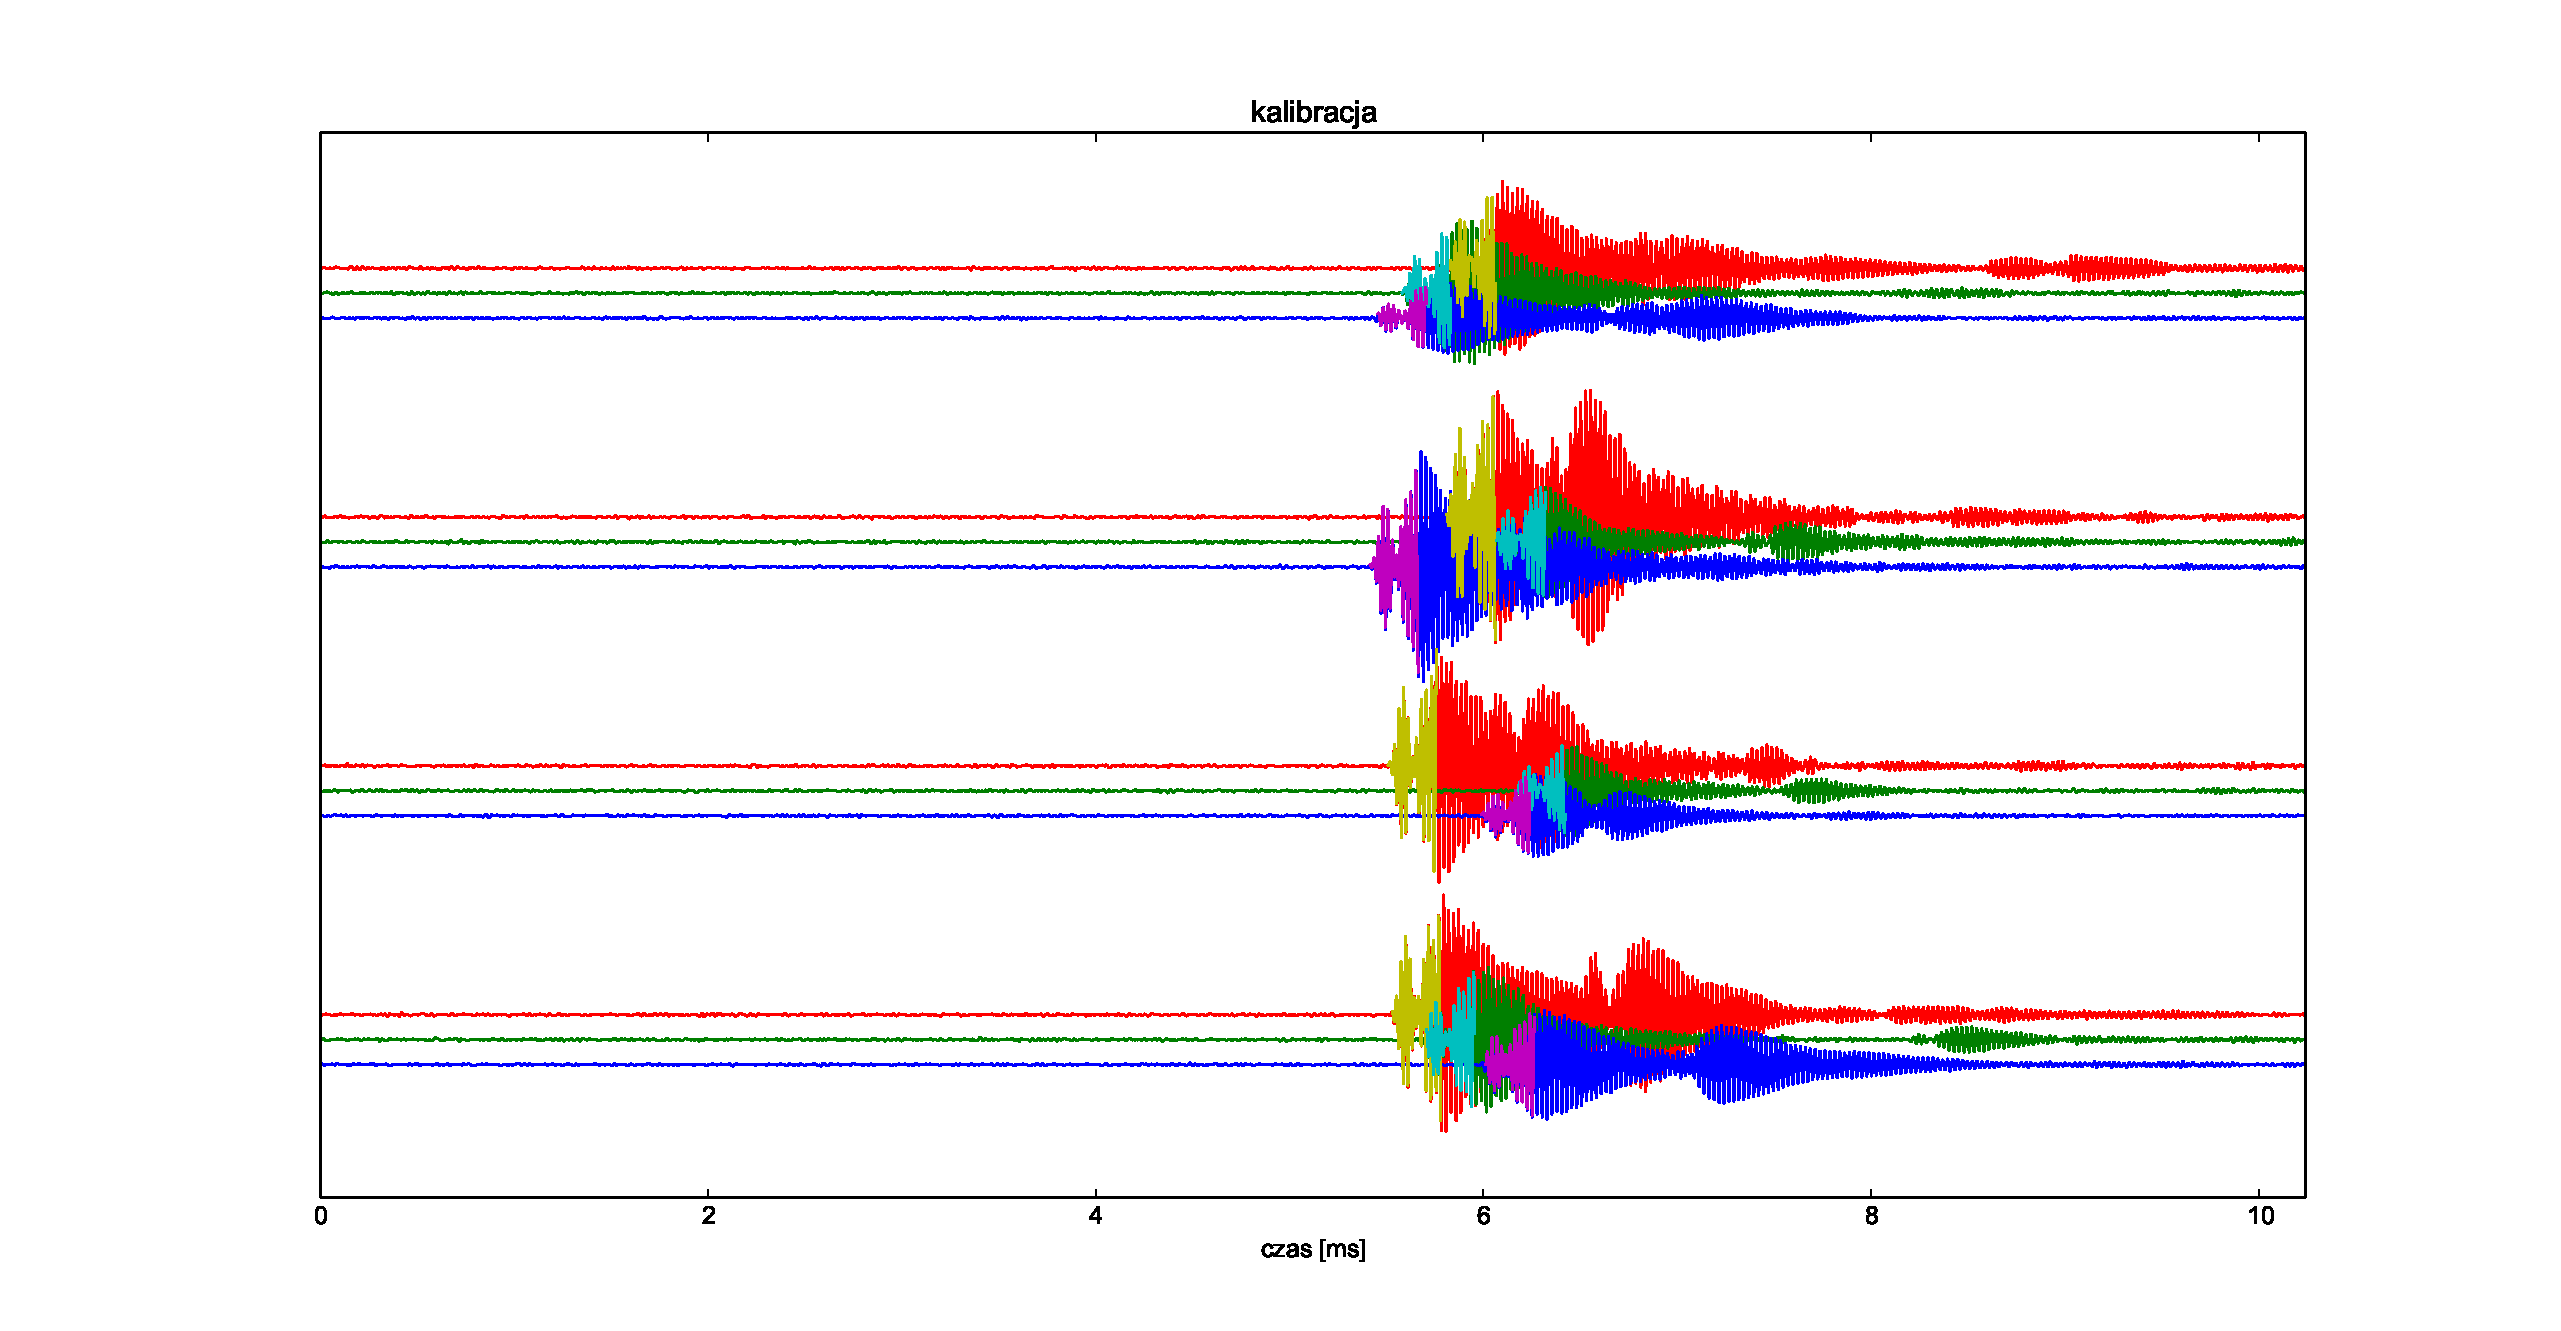
\includegraphics[width=1.12\textwidth, trim= 46mm 0mm 0mm 0mm,clip]{kalibracja_12x}
    \caption{Kalibracja, widok 12 sygnałów z zaznaczonymi \textit{wzorcami}}
    \label{fig:kalibracja_12x}
\end{figure}

\newpage

\section{Obsługa programu \textit{scan.py}}

Do obsługi prototypu służy program \textit{scan.py}. Po jego uruchomieniu 
na monitorze wyświetlają się trzy okna: 
\begin{itemize}
 \item widok 3D, na którym zaznaczona jest 
pozycja nadajnika, cztery punkty reprezentujące głośniki nadajnika oraz trzy wektory normalne reprezentujące 
jego orientację jak i położenie, rysunek \ref{fig:widok3d}
 \item widok 2D, na którym przedstawiono nałożone na siebie dwa rzuty prostopadłe nadajnika na płaśczyzny XY i XZ, rysunek \ref{fig:widok2d}
 \item widok mocy sygnału, który informujący o sile odbieranego sygnału oraz o błędzie pomiędzy \textit{wzorcem} a odebranym sygnałem, rysunek \ref{fig:power}
\end{itemize}

[TODO]
Głównym oknem program jest widok 3D, na którym przedstawiono położenie nadajnika w przestrzeni,
wszelkie zmiany położenia nadajnika automatycznie odświeżają wszystkie widoki. Podczas uruchamiania programu
aktualne położenie nadajnika przyjmowane jest jako początek układu współrzędnych.
Jeśli któryś z głośników straci widoczność z mikrofonami obraz przestaje się odświeżać, a informacja dlaczego tak
się dzieje widoczna jest na widoku mocy sygnału.

Dla celów demonstracyjnych istnieje możliwość rysowania (stawiania punktów) w przestrzeni. Aby zapamiętać punkty
należy wcisnąć klawisz "p", aby zapisać wynik rysowania należy wcisnąć klawisz "s", do wyczyszczenia obrazu służy klawisz "c".
Rysunek [TODO] przedstawia przykładowy rysunek w przestrzeni.


\rysunek{3d}{Widok 3D}{\label{fig:widok3d}}
\rysunek{2d}{Widok 2D}{\label{fig:widok2d}}
\rysunek{power}{Widok informujący o mocy sygnału oraz błędzie pomiędzy \textit{wzorcem} a sygnałem}{\label{fig:power}}

